% ==============================================================================
% =================================== Einleitung ================================
% ==============================================================================

\chapter{Einleitung}
\label{chap:einleitung}
\thispagestyle{fancy}

\section{Hintergrund und Zielsetzung}

Die vorliegende Arbeit beschäftigt sich mit der explorativen Datenanalyse, der Anwendung von Machine-Learning-Verfahren sowie der Konzeption von Big-Data-Architekturen. Grundlage bilden die Studieninhalte der Module \textit{Explorative Datenanalyse} \cite{1}, \textit{Machine Learning} \cite{2} und \textit{Big Data Architektur} \cite{3} von Thomas Tilli an der Wilhelm Büchner Hochschule. Ziel ist es, die theoretischen Inhalte dieser Module praktisch umzusetzen und die gewonnenen Erkenntnisse in Form eines reproduzierbaren Analyse-Workflows zu dokumentieren.

Die Arbeit gliedert sich in drei Hauptteile:

\begin{enumerate}
    \item \textbf{Explorative Analyse} eines Film-Datensatzes (\textit{2019}) mit den Schwerpunkten Datenbereinigung, deskriptive Statistik und Visualisierung.
    \item \textbf{Regressions- und Klassifikationsverfahren} auf Basis des California-Housing- und Wine, einschließlich Modellbewertung und Hyperparameteroptimierung.
    \item \textbf{Clusteranalyse} und Dimensionsreduktion mit dem Wine-Datensatz sowie Einordnung in den Kontext von \acs{NoSQL}-Datenbanken und Streaming-Architekturen.
\end{enumerate}

\section{Wissenschaftliche Arbeitsumgebung}

Für die Umsetzung aller Analysen wird eine konsistente, reproduzierbare Entwicklungsumgebung aufgebaut. Die Wahl der Software-Infrastruktur orientiert sich an den in den Studienheften empfohlenen Tools, wird jedoch aufgrund der aktuellen Entwicklungen im Open-Source-Ökosystem präzisiert.

\subsection{Betriebssystem und Basis-Installation}

Die gesamte Analyse wird unter \textbf{Windows 11} (\textit{Version 22H2}) durchgeführt. Als grundlegende Voraussetzung für die Analyseumgebung wird \textbf{Python} in der Version 3.12 installiert.

\subsubsection{Python-Installation}

Als grundlegende Voraussetzung für die gesamte Analyseumgebung wird \textbf{Python} in einer Version $\ge$ 3.9 benötigt. Für Windows-Systeme wird die Installation von Python über die offizielle Webseite\footnote{\url{https://www.python.org/downloads/}} empfohlen.

\paragraph{\textbf{Wichtiger Hinweis: PATH-Umgebungsvariable}}

Es ist \textbf{erforderlich}, dass das Python-Verzeichnis in der \texttt{PATH}-Umgebungsvariable des Systems eingetragen ist. Nur so können Python- und \acs{pip}-Befehle von jedem beliebigen Ort in der Kommandozeile oder PowerShell ausgeführt werden.

Bei der Installation über den \textbf{offiziellen Installer} von \url{https://www.python.org/downloads/} ist daher unbedingt die Option \texttt{Add Python to PATH} am unteren Rand des Installationsfensters zu aktivieren (\textit{siehe Abbildung \ref{fig:python_path}}). Diese Option ist standardmäßig \textbf{nicht} aktiviert, was bei unerfahrenen Anwender:innen häufig zu Fehlermeldungen wie \textit{"python is not recognized as an internal or external command"} führt.

\begin{figure}[h]
    \centering
    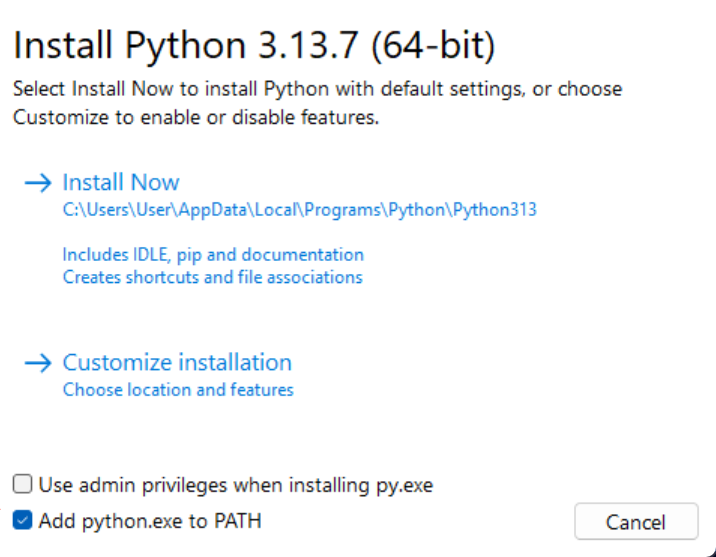
\includegraphics[width=0.9\textwidth]{./asset/image/PythonInstallerPath.png}
    \caption{Installationsfenster des offiziellen Python-Installers (\textit{Quelle: Eigene Aufnahme)}}
    \label{fig:python_path}
\end{figure}

Alternativ kann Python auch direkt über die PowerShell installiert werden – ein Verfahren, das besonders für automatisierte Setups oder für Nutzer ohne Administratorrechte geeignet ist. Die Installation erfolgt dabei über den integrierten Paketmanager \texttt{\acs{winget}} (\textit{siehe Listing \ref{lst:winget}}):

\lstinputlisting[
    language=bash, 
    caption={Python-Installation unter Windows per PowerShell}, 
    label={lst:winget}
]{asset/code/PythonInstallation.tex}

Bei der Installation über \texttt{\acs{winget}} wird die PATH-Konfiguration automatisch vorgenommen. Sollte dennoch eine Fehlermeldung auftreten, kann der Pfad manuell über die Systemeinstellungen hinzugefügt werden (\textit{siehe Listing \ref{lst:path_manual}}):

\lstinputlisting[
    language=bash, 
    caption={Manuelles Hinzufügen von Python zum PATH (\textit{PowerShell})}, 
    label={lst:path_manual}
]{asset/code/PythonInstallationII.tex}

Nach erfolgreicher Installation und korrekter PATH-Konfiguration kann das System mit der Einrichtung der Conda-Umgebung fortfahren. Der Einsatz von \texttt{\acs{virtualenv}} mit \texttt{\acs{pip}} wäre eine alternative, leichtgewichtige Lösung. Im Rahmen dieser Arbeit wird jedoch Conda bevorzugt, da es systemnahe Abhängigkeiten auf Windows-Systemen zuverlässiger auflöst.

\paragraph{\textbf{Anmerkung zur Python-Installation}}

Die systemweite Installation von Python ist für die Nutzung von Conda-Umgebungen technisch nicht zwingend erforderlich, da Conda eigenständige Python-Interpreter in den jeweiligen Umgebungen bereitstellt. Dennoch wird in dieser Arbeit eine systemweite Python-Installation vorgenommen, um eine konsistente Basis für die Entwicklungsumgebung zu schaffen und die Nutzung von Python-Werkzeugen außerhalb der Conda-Umgebungen zu ermöglichen. Dieser Schritt entspricht der gängigen Praxis in Data-Science-Projekten, bei denen häufig sowohl eine systemweite Python-Installation als auch isolierte Conda-Umgebungen zum Einsatz kommen.

\subsubsection{Miniforge-Installation}

Als Paketmanager und Umgebungsverwaltung kommt \textbf{Miniforge}\footnote{\url{https://conda-forge.org/download/}}\footnote{\url{https://github.com/conda-forge/miniforge}} zum Einsatz. Eine schlanke Conda-Distribution, die standardmäßig den Community-Kanal \texttt{conda-forge} verwendet. Diese Entscheidung basiert auf folgenden Erwägungen:

\begin{itemize}
    \item \textbf{Aktualität der Pakete:} \texttt{conda-forge} bietet gegenüber dem offiziellen Anaconda-Kanal deutlich aktuellere Versionen von Data-Science-Bibliotheken wie \texttt{pandas}, \texttt{scikit-learn} oder \texttt{seaborn}.
    \item \textbf{Umfangreiches Paketangebot:} Mit über 30.000 Paketen deckt \texttt{conda-forge} praktisch alle für diese Arbeit benötigten Abhängigkeiten ab.
    \item \textbf{Open-Source-Transparenz:} Die Pakete werden von der Community gepflegt und unterliegen keinen kommerziellen Lizenzbeschränkungen, wie sie bei der Anaconda-Distribution ab 2020 für Unternehmen eingeführt wurden.
    \item \textbf{Optimierung für Data Science:} \texttt{conda} löst systemnahe Abhängigkeiten (\textit{\acs{z. B.} \acs{BLAS}-Bibliotheken für \acs{NumPy}}) zuverlässig und plattformunabhängig auf, was bei \texttt{\acs{pip}} häufig zu Kompilierproblemen führen kann.
\end{itemize}

Nach der Installation ist es wichtig, die Miniforge-Umgebung zu aktivieren. Unter Windows geschieht dies über den \textbf{Miniforge Prompt}, der im Startmenü unter \texttt{Miniforge3} zu finden ist. Für fortgeschrittene Anwender oder automatisierte Setups kann die Miniforge-Umgebung auch manuell über die System-Eingabeaufforderung aktiviert werden. Die Aktivierung erfolgt durch direkten Aufruf des Aktivierungs-Skripts:

\lstinputlisting[
    language=bash, 
    caption={Pfad zum Miniforge Prompt unter Windows}
]{asset/code/Miniforge.tex}

Der Miniforge Prompt ist eine speziell konfigurierte PowerShell- oder Eingabeaufforderung, in der alle \texttt{conda}-Befehle ohne weitere Konfiguration verfügbar sind. Wird stattdessen eine reguläre PowerShell oder Eingabeaufforderung geöffnet, sind die \texttt{conda}-Befehle zunächst nicht verfügbar, da die erforderlichen Umgebungsvariablen nicht gesetzt sind.

\subsection{Projektstruktur}

Vor der Einrichtung der isolierten Entwicklungsumgebung wird eine klare Projektstruktur definiert. Dies gewährleistet eine saubere Trennung zwischen der Conda-Umgebung (\textit{den Werkzeugen}) und den eigentlichen Arbeitsdateien (\textit{Notebooks}, \textit{Daten}, \textit{Code}).

Die folgende Ordnerstruktur wird für dieses Projekt angelegt:

\begin{figure}[h]
    \centering
    \begin{forest}
        for tree={
            font=\ttfamily,
            grow'=0,
            child anchor=west,
            parent anchor=south,
            anchor=west,
            calign=first,
            edge path={
                \noexpand\path [draw, \forestoption{edge}] (!u.south west) +(10pt,0) |- node[fill,inner sep=1.5pt] {} (.child anchor)\forestoption{edge label};
            },
            before typesetting nodes={
                if n=1{
                    insert before={[,phantom,calign with current]}
                }{}
            },
            fit=band,
            before computing xy={l=22pt},
        }
        [\textbf{C:}\textbackslash \textbf{Users}\textbackslash \textbf{USER}\textbackslash
            [\textbf{miniforge3}\textbackslash $\leftarrow$ \textit{Conda-Installation}
                [\textbf{envs}\textbackslash
                    [\textbf{B-BIDA01XX}\textbackslash $\leftarrow$ \textit{Isolierte Conda-Umgebung}]
                ]
            ]
            [\textbf{B-BIDA01XX}\textbackslash $\leftarrow$ \textbf{\textit{Projektordner}}
                [\textbf{data}\textbackslash
                    [\textbf{movies2019.csv}]
                    [\textbf{california\_housing.csv}]
                    [\textbf{wine.csv}]
                ]
                [\textbf{notebooks}\textbackslash
                    [\textbf{Aufgabe\_1\_Explorative\_Analyse.ipynb}]
                    [\textbf{Aufgabe\_2\_Regression\_Klassifikation.ipynb}]
                    [\textbf{Aufgabe\_3\_Clustering.ipynb}]
                ]
                [\textbf{output}\textbackslash $\leftarrow$ \textit{Exportierte Grafiken}]
            ]
        ]
    \end{forest}
    \caption{Projektstruktur des Analyse-Workflows (\textit{Quelle: Eigene Darstellung})}
    \label{fig:project_structure}
\end{figure}

Die Trennung zwischen Conda-Umgebung und Projektordner ermöglicht eine saubere Isolation der Systemabhängigkeiten vom eigentlichen Arbeitsmaterial. Die Umgebung kann somit für andere Projekte wiederverwendet oder bei Bedarf neu erstellt werden, ohne die Arbeitsdateien zu beeinflussen.

\subsection{Erstellung der isolierten Umgebung}

Für jedes Teilprojekt wird eine eigene Conda-Umgebung angelegt, um Konflikte zwischen verschiedenen Paketversionen zu vermeiden. Die Umgebung für die vorliegende Arbeit wird mit folgendem Befehl initialisiert (\textit{siehe Listing \ref{lst:conda_install}}):

\lstinputlisting[
    language=bash, 
    caption={Erstellen und Aktivieren der Conda-Umgebung}, 
    label={lst:conda_install}
]{asset/code/CondaForge.tex}

\paragraph{\textbf{Wichtiger Hinweis: Aktivierung der Umgebung}}

Alle Installationen sind in der \textbf{aktiven} Conda-Umgebung durchzuführen. Die aktive Umgebung ist am Prompt erkennbar: \texttt{(\textit{B-BIDA01XX})} zeigt an, dass die Projekt-Umgebung aktiv ist, während \texttt{(\textit{base})} die Standard-Umgebung kennzeichnet (\textit{siehe Listing \ref{lst:conda_install_ii}}).

\lstinputlisting[
    language=bash, 
    caption={Korrekte Aktivierung vor der Installation}, 
    label={lst:conda_install_ii}
]{asset/code/CondaForgeII.tex}

Nach Bestätigung der Abhängigkeiten werden die erforderlichen Pakete aus dem \texttt{conda-forge}-Kanal heruntergeladen und in der Umgebung installiert. Die Installation umfasst neben Python 3.12 auch die erforderlichen systemnahen Abhängigkeiten wie \acs{OpenSSL}, \acs{SQLite} und die Microsoft Visual C++ Redistributable, die für die Ausführung von Data-Science-Paketen unter Windows notwendig sind. Anschließend werden die benötigten Bibliotheken installiert (\textit{siehe Listing \ref{lst:conda_install_iii}}):

\lstinputlisting[
    language=bash, 
    caption={Installation der Data-Science-Bibliotheken}, 
    label={lst:conda_install_iii}
]{asset/code/CondaForgeIII.tex}

Zusätzlich kommen für spezifische Aufgaben folgende Pakete hinzu:

\begin{itemize}
    \item \texttt{statsmodels} für erweiterte statistische Tests
    \item \texttt{scipy} für wissenschaftliche Berechnungen
    \item \texttt{missingno} für die Visualisierung fehlender Werte
\end{itemize}

Alle Installationen erfolgen ausschließlich über den \texttt{conda-forge}-Kanal, was durch folgende Konfiguration sichergestellt wird:

\lstinputlisting[
    language=bash, 
    caption={Konfiguration des conda-forge-Kanals}
]{asset/code/CondaForgeIV.tex}

\subsection{Arbeitsumgebung: Jupyter Notebook}

Die gesamte Code-Entwicklung und Dokumentation erfolgt in \textbf{Jupyter Notebooks}. Dieses interaktive Werkzeug ermöglicht eine enge Verzahnung von ausführbarem Python-Code, visuellen Ausgaben und erklärendem Markdown-Text, eine ideale Voraussetzung für die explorative Datenanalyse und die Nachvollziehbarkeit der Ergebnisse.

Der Jupyter-Server wird nach der Aktivierung der Conda-Umgebung mit folgendem Befehl gestartet:

\lstinputlisting[
    language=bash, 
    caption={Starten des Jupyter-Servers}
]{asset/code/JupyterServers.tex}

Nach der Ausführung des Befehls öffnet sich automatisch ein Browserfenster mit der Jupyter-Oberfläche. Der Server läuft lokal auf \texttt{http://localhost:8888} und ermöglicht das Erstellen, Bearbeiten und Ausführen von Notebooks.

\begin{figure}[h]
    \centering
    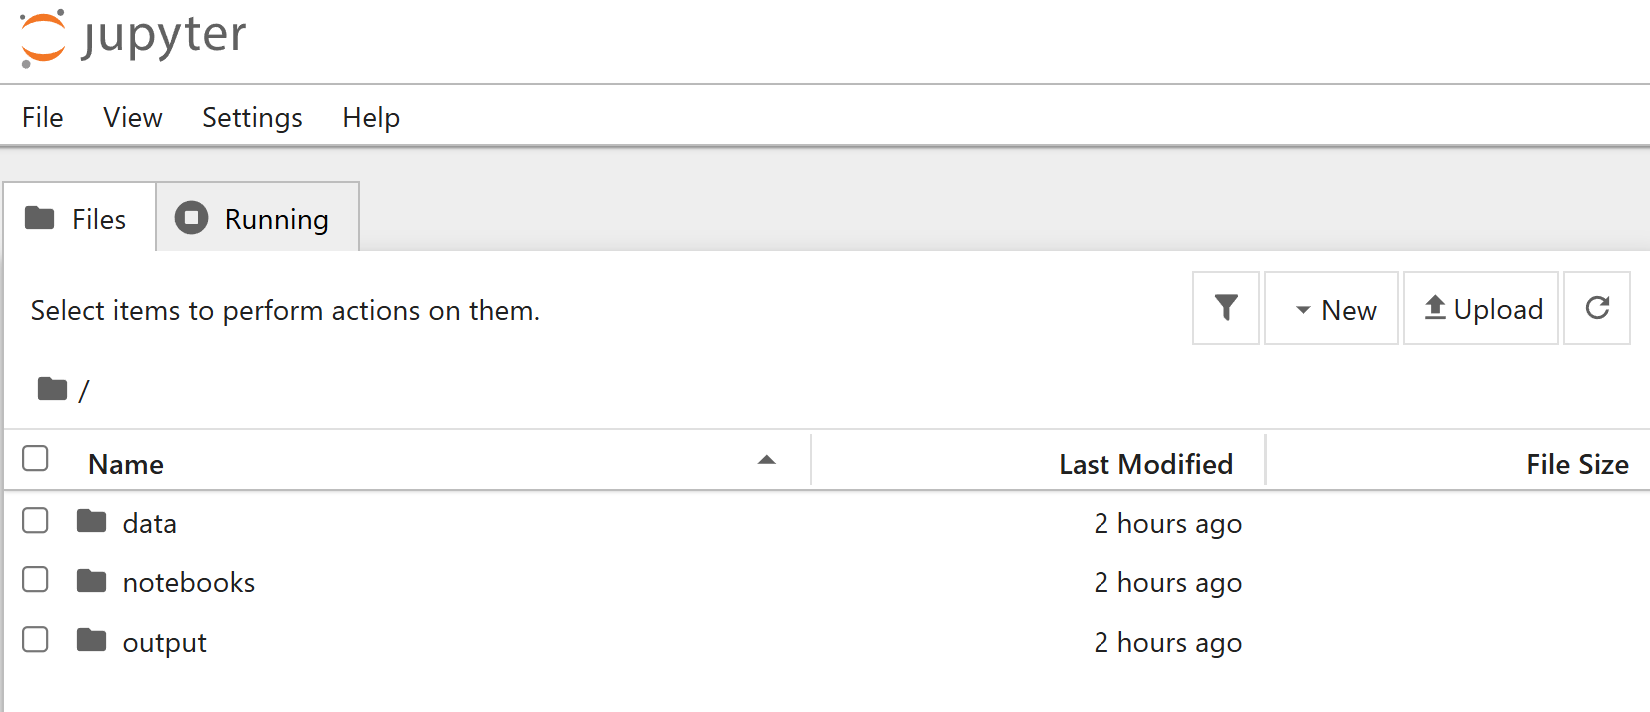
\includegraphics[width=0.9\textwidth]{./asset/image/JupyterServers.png}
    \caption{Jupyter-Dashboard nach dem Start des Servers (\textit{Quelle: Eigene Aufnahme})}
    \label{fig:jupyter_servers}
\end{figure}

Die Notebooks werden nach folgendem Muster strukturiert:

\begin{enumerate}
    \item \textbf{Importe und Konfiguration} (\textit{alle erforderlichen Bibliotheken})
    \item \textbf{Daten laden und erste Inspektion} (\texttt{\textit{head()}}, \texttt{\textit{info()}}, \texttt{\textit{describe()}})
    \item \textbf{Datenaufbereitung} (\textit{Umgang mit fehlenden Werten}, \textit{Umcodierung}, \textit{Skalierung})
    \item \textbf{Explorative Visualisierung} (\textit{Box-Plots}, \textit{Histogramme}, \textit{Pair-Plots}, \textit{Korrelationsmatrizen})
    \item \textbf{Modellierung} (\textit{Training}, \textit{Evaluation}, \textit{Hyperparameter-Optimierung})
    \item \textbf{Interpretation und Diskussion} der Ergebnisse
\end{enumerate}

Diese Struktur folgt dem in \cite{2} beschriebenen \emph{Epizyklus der Datenanalyse} und gewährleistet eine systematische Vorgehensweise.

\section{Aufbau der Arbeit}

Im weiteren Verlauf werden die drei Einsendeaufgaben der Module BID02, BID03 und BID04 Schritt für Schritt bearbeitet. Die Lösungen sind vollständig in Python implementiert und werden jeweils mit den dazugehörigen Code-Auszügen, Visualisierungen und Ergebnisinterpretationen dokumentiert.

% ==============================================================================
% =============================== Ende Einleitung ===============================
% ==============================================================================